\documentclass[a4paper, 12pt]{article}

\usepackage[utf8]{inputenc}
\usepackage{amsmath}
\usepackage{cite}
\usepackage{indentfirst}
\usepackage{listings}
\usepackage{graphicx}
\usepackage[colorinlistoftodos]{todonotes}
\usepackage{tikz}
\usepackage{url}
\usepackage{enumerate}
\usepackage{float}
\usepackage{ragged2e}
\usetikzlibrary{calc,patterns,angles,quotes}

%Usage: \btable{table specs}{caption}{reference label}



\begin{document} %Comeco do documento

\begin{titlepage}

\begin{figure}[H]
\centering

\includegraphics[width=1.75cm]{IFSC_USP.png} % Nome da Imagem

\end{figure}
    \begin{center}
        Universidade de São Paulo \\

        Instituto de Física de São Carlos \\


\vspace{10pt}


        \vspace{85pt}


         \large\textbf{{Prática 5: Dinâmica Populacional }} % Titulo da Pratica
        \vspace{160pt}

    \end{center}

    \begin{flushright}

         Stefan Taiguara Couperus Leal 10414866\\ % Colocar os nomes dos alunos aqui
    \end{flushright}

    \begin{center}
        \vspace{\fill}
        Maio de 2019 % Onde eu coloco a data
    \end{center}
\end{titlepage}

\newpage
%\tableofcontents    % Posso ativar para ter a tabela de conteudo

\thispagestyle{empty}

\newpage
\pagenumbering{arabic}

\justifying
\tableofcontents

\newpage

\section{Introdução}
A equação diferencial que será foi utilizada para descrever o crescimento populacional é:

\begin{equation}
    d N(t) = \alpha N(t) dt
    \label{eq:first}
\end{equation}

Sendo $\alpha$ uma constante de crescimento/decrescimento populacional. Observando a equação acima percebe-se que não é muito realístico, já que prevê um crescimento exponencial sem limites (há uma ausência de predadores, falta de recursos, mortalidade dos indivíduos, etc).

Para uma descrição mais exata do fenômeno é um imposto um corte quando o valor atingir um certo $N_{max}$.

O objetivo da pratica é estudar as condições que um dado um valor inicial para o numero N de indivíduos permaneça constante com o tempo.


O estudo do mapeamento vai revelar uma grande complexidade e dependência sensível das condições iniciais, definindo um comportamento caótico que será observado nos exercícios.


Primeiramente foi discretizada a equação  \ref{eq:first}, ou seja, foi considerado instantes de tempo $t$ e $t + \Delta t$ (sendo $\Delta t$ fixo, mas não necessariamente pequeno). A equação fica:

\begin{equation}
    N_{i + 1} = (1 + \alpha \Delta t) N_i \approx r N_i
\end{equation}

Sendo $r = 1 + \alpha \Delta t > 1$. Depois disso foi imposto um limite de $N_max$.

\begin{equation}
    N_{i + 1} = r N_i ( 1 - \frac{N_i}{N_{max}} )
\end{equation}

Para uma mais simples visualização foi adotado $x_i \approx \frac{N_i}{N_{max}}$. Gerando a equação utilizada para a simulação.

\begin{equation}
    x_{i + 1} = r x_i (1 - x_i)
    \label{eq:main}
\end{equation}

A equação \ref{eq:main} define um mapeamento. Neste projeto será estudo a evolução do mapa G(x), o chamado mapa logístico.

\section{Metodologia Aplicada}


\subsection{Tratamento Geral}

A inteção desta prática é encontrar valores de $G(x)$ para quais $G(x^*) = x^*$.

Será observado as propriedades de G(x), que são:

\begin{itemize}
	\item $x^* = 0$ Sempre deve ser uma solução \label{item:i}
	\item $r$ deve estar sempre entre 1 e 4. \label{item:ii}
	\item Dado que  $ 0 \leq r \leq 4 $, Há uma solução para  $x^*$ ? \label{item:iii}
\end{itemize}

Portanto será variado o valor de $r$ (observando o valor de convergência) afim de verificar as propriedades listadas acima.

\subsection{Rumo ao Caos}


Não basta ser um ponto fixo do mapa $G(x)$ para um valor de x ser estável na evolução da população.
O que ocorre para pontos fixos depende da estabilidade do ponto, que depende do valor do parâmetro $r$. Para $r > 3$ (e $r < 3.5$) o ponto fixo $x^{!}$ torna-se instável, levando a um comportamento oscilatório entre $x_1$ e $x_2$. 

Será realiza testes da evolução do sistema, aumentando o valor de $r$. Será procurado ver o fenômeno de duplicação de período (que deve ser  observado logo antes do caos). Portanto será observado a formação do caos e anotando os valores de $r$ onde as duplicações ocorrem. Com isso será calculado a constante de Feigenbaum $\delta$ pela equação abaixo:

\begin{equation}
	\delta = \frac{r_2 - r_1}{r_3 - r_2}
	\label{eq:deltaDelta}	
\end{equation}

\subsection{O Caos!}


Como foi visto que o sistema evoluirá para o caos a medida que o valor de r for aumentando, vai ser
implementado o calculo do expoente de Lyapunov (é uma forma de quantificar o a falta de controle que tem
sobre um numero inicial $x_0$). Será observado a sensibilidade das condições iniciais colocando o
$x_0$ de dois sistemas variando por um $\epsilon$, desta forma será observado a diferença dos dois sistemas.


Afim de obter o expoente de Lyapunov será utilizado de dois métodos:


Serão simulados dois sistemas: $G^{i}(x_0)$  e $G(x_0^{i} + \epsilon)$.

O primeiro é:  cada interação será calculado a distância $d$ utilizando da equação \ref{eq:distancia}, com
isso será observado o comportamento do gráfico e será extraído o  expoente de Lyapunov ($\gamma$).

\begin{equation}
  d(i) = | G(x_0^{i} + \epsilon) - G(x_0^{i})|
  \label{eq:distancia}
\end{equation}


A simulação será realizado para valores $r <  3.0$ , $ r > 3.6$.


A outra forma de estimar a constante de Lyapunov é supor um comportamento exponencial para d, com o tempo
relacionado com a derivada do mapa $G^{(i)}(x)$ (nota-se que o valor de $\epsilon$ é minimo). Como essas considerações obtêm-se:

\begin{equation} 
  \lambda = \frac{1}{n - 1} \sum_{j = 0}^{n - 1} \ln | G^{'} (x_j) | 
  \label{eq:lambda_intermediary}
\end{equation}

Resolvendo o $G^{'}(x_j)$ temos:

\begin{equation} 
  \lambda = \frac{1}{n - 1} \sum_{j = 0}^{n - 1} \ln|r (1 - 2 x) |
  \label{eq:lambda}
\end{equation}



\section{Resultados Obtidos}

\subsection{Tratamento Geral}

O programa usado para chegar nos resultado esta abaixo, ja para graficar foi utlizado do gnuplot. 

\lstset{language=FORTRAN}
\begin{lstlisting}
program crescimento
implicit none

real(8) :: G, r, x1, x0
integer :: i, N

N = 1000

print *, "Valor de x_o: "
read *, x0
print *, "Valor de r: "
read *,  r


open(1, file="exponential.dat")
x = x0
do i = 0, N, 1
x1 = r * x0 * (1.0d0 - x0)
xo = x

write(1 , *) i, x0, x1
enddo
close(1)

end program crescimento


\end{lstlisting}

\hspace{0.5cm}

\subsubsection{Para r = 1}

	Usando do programa citado acima foi calculado para $ r = 1$, com isso tem-se que:
	
%Como colocar figuras
\begin{figure}[H]
	\centering
	\caption{Crescimento Populacional para r = 1}{}
	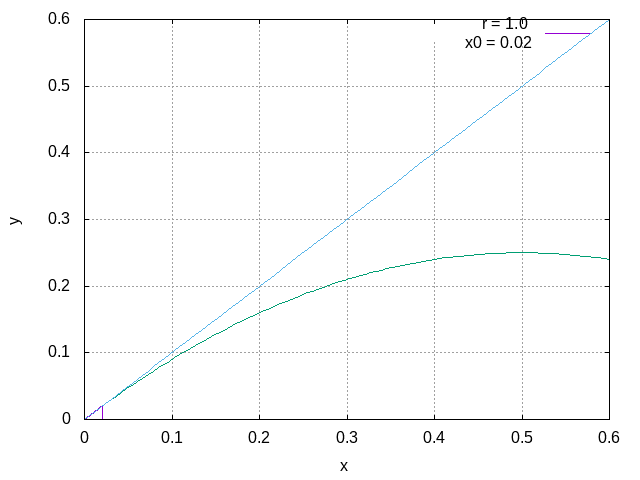
\includegraphics[width=10.0cm]{r=1_0__x0=0_02.png}
	\label{fig:img1}
\end{figure}

Na figura \ref{fig:img1} pe notado que não há valor de convergência, onde o único valor no qual $G(x^{*}) = x^{*}$ é para $G(0)$. 

\hspace{0.5cm}

\subsubsection{Para r = 2}
\begin{figure}[H]
	\centering
	\caption{Crescimento Populacional para r = 2}{}
	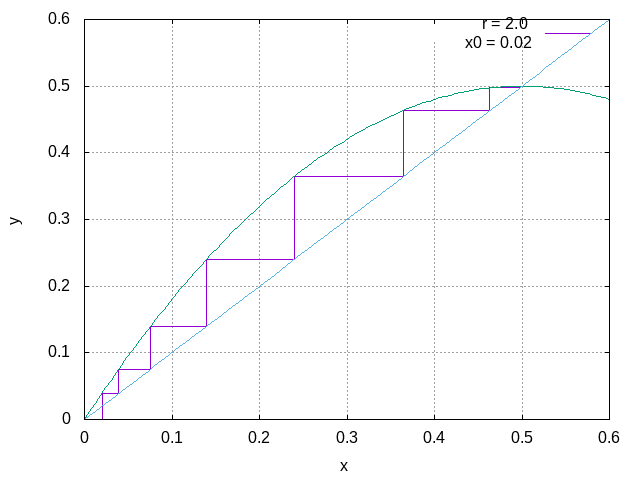
\includegraphics[width=10.0cm]{r=2_0__x0=0_02.png}
	\label{fig:img2}
\end{figure}

É notado que há uma convergência para um único ponto, sendo o valor dele igual a:

\begin{equation*}
	x^{*} = 0.50000000000000008
\end{equation*}


\hspace{0.5cm}

Percebe-se também que o primeiro item das propriedades citadas  em \ref{item:i} é válido, já que $G(0) = 0$.

\hspace{0.5cm}

\subsubsection{Para r = 2.5}

\begin{figure}[H]
	\centering
	\caption{Crescimento Populacional para r = 2.5}{}
	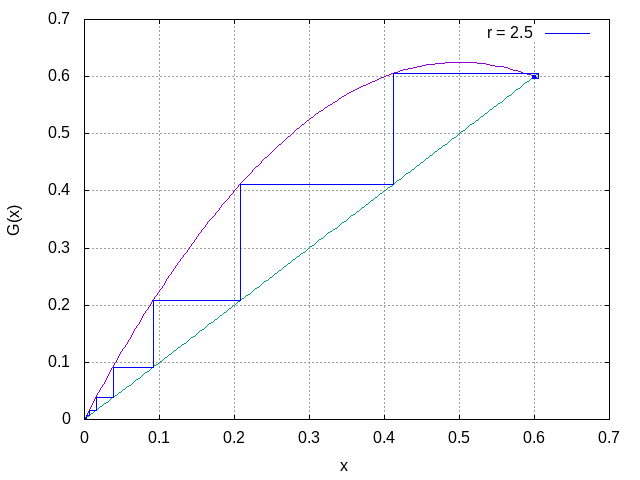
\includegraphics[width=10.0cm]{r=2_5.png}
	\label{fig:img2.5}
\end{figure}

O valor de convergência onde $G(x^{*}) = x^{*} $  é:

	
\hspace{0.5cm}

\begin{equation*}
	  x^{*} = 0.60000000000000009
\end{equation*}

\hspace{0.5cm}

\subsubsection{Para r = 3}

\begin{figure}[H]
	\centering
	\caption{Crescimento Populacional para r = 3}{}
	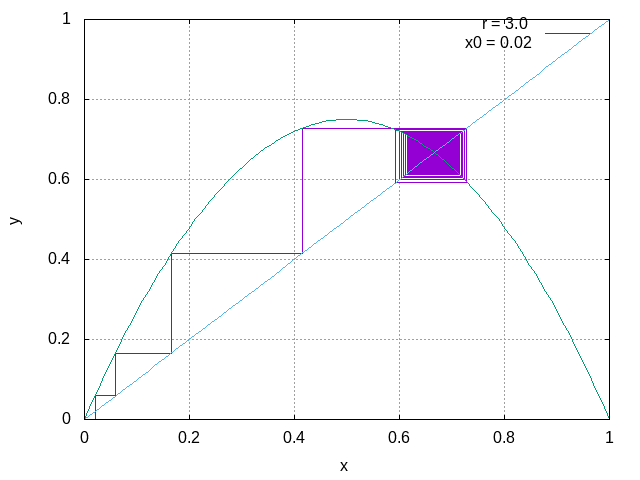
\includegraphics[width=10.0cm]{r=3_0__x0=0_02.png}
		\label{fig:img3}
\end{figure}

O valor de convergência é de: 


\begin{equation*}
	x^{*} = 0.66430218085545800
\end{equation*}


\hspace{0.5cm}

\subsubsection{Para r = 3.545}

\begin{figure}[H]
	\centering
	\caption{Crescimento Populacional para r = 3.545}{}
	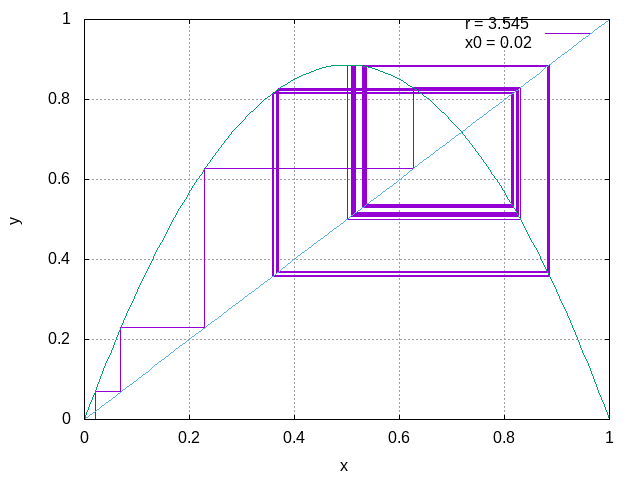
\includegraphics[width=10.0cm]{r=3_545__x0=0_02.png}
	\label{fig:img4}
\end{figure}

\hspace{0.5cm}

Ja na figura \ref{fig:img4} é notado que há dois valores onde oa função oscila. Sendo estes valores igual a:

\begin{equation*}
	x_1 =  0.53030632825343749	
\end{equation*}

\begin{equation*}
 x_2 = 0.88299401132833288
\end{equation*}

\hspace{0.5cm}


\subsubsection{Para r = 4}

\begin{figure}[H]
	\centering
	\caption{Crescimento Populacional para r = 4.0}{}
	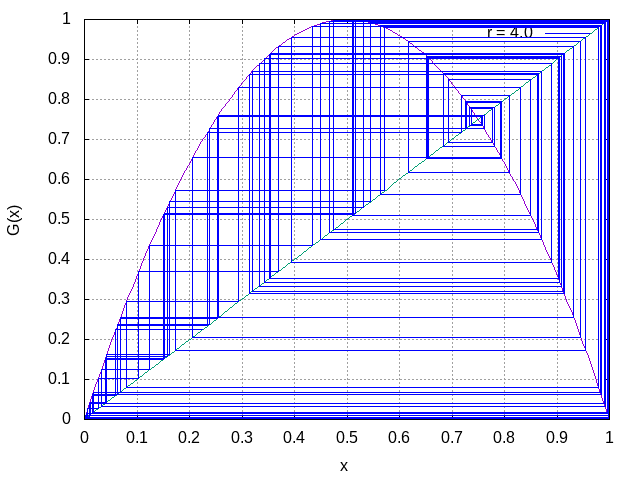
\includegraphics[width=10.0cm]{r=4.png}
	\label{fig:img5}
\end{figure}


Percebe que o crescimento populacional atingiu um padrão caótico, onde não se é possível determinar valor de convergência.



\subsection{Rumo ao Caos}

O programa usado para observar o comportamento da variação de $r$ afim de descobrir a constante de Feigenbaum se encontra abaixo: 

\begin{lstlisting}
program rvariation
implicit none

real(8) :: r, dr, x0, x1
real(8) :: r_min, r_max

integer :: contador, verificador

integer :: i, n_test, n_steps, r_steps
r_min = 1.0d0
r_max = 4.0d0

n_test = 100
n_steps = 1000
r_steps = 1000


contador = 1
verificador = 0

open(1, file='rVariation.dat')

dr = (r_max - r_min) / r_steps ! Incremento em r

r = r_min

do while ( r < r_max)
	x0 = 0.5d0
	
	do i = 1, n_test, 1
		x1 = r * x0 * (1.d0 - x0)
		x0 = x1
	enddo
	
	do i = 1, n_steps, 1
		x1 = r * x0 * (1.d0 - x0)
		write(1, *) r, x1
	
		x0 = x1
	enddo
	
	r = r + dr
enddo
close(1)

end program rvariation

\end{lstlisting}


\begin{figure}[H]
	\centering
	\caption{Diagrama de bifurcação em função de $r$}{}
	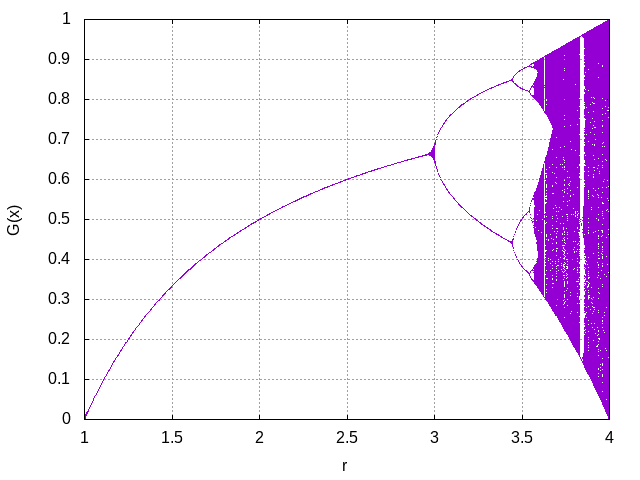
\includegraphics[width=10.0cm]{lambda.png}
	\label{fig:firstlambda}
\end{figure}
 

Para fins de analise foi pego só os valores depois de $ r = 2.8$ (já que antes desse intervalo não há bifurcação).
 
\begin{figure}[H]
	\centering
	\caption{Diagrama de bifurcação em função de $r$}{}
	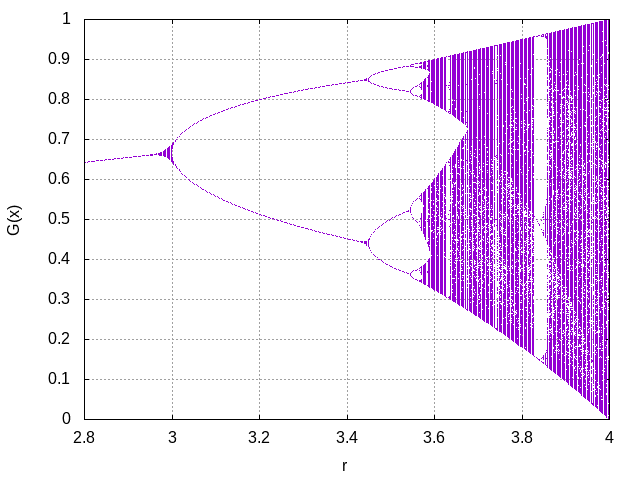
\includegraphics[width=10.0cm]{lambdaCloser.png}
	\label{fig:lambda}
\end{figure}
 
 
 Com isso os valores de $r$ são:
 
$r_1 = 3.4485$

$r_2 = 3.5438$

$r_3 = 3.5644$


\hspace{0.5cm}

Utilizando da equação \ref{eq:deltaDelta}:

\hspace{0.5cm}

\centering $\delta = 4.6262$.

\hspace{0.5cm}
	
	
Comparando o valor obtido pelo da literatura \cite{wiki}.

\begin{equation*}
  \frac{4.6262}{4.6692} \approx 0.99
\end{equation*}



\subsection{O Caos!}

O programa usado para calcular o valor do expoente de Lyapunov é:

\hspace{0.5cm}

\begin{lstlisting}
program exer1
implicit none

! Declaracao de variaveis
integer :: i, N

real(8) :: r, epsilon
real(8) :: x0, x1, x0t, x1t

real(8) :: lambda, x0d, x1d


read *, r
read *, x0
read *, epsilon


N = 1000
x0t = x0 + epsilon
x0d = x0

open(1, file="dist_out.dat")
write(1, *) 0, x1, x1t, abs(x1 - x1t)

do i = 1, N, 1

! Parte A
x1 = r * x0 * (1.d0 - x0)
x1t = r * x0t * (1.d0 - x0t)

write(1, *) i, x1, x1t, abs(x1 - x1t)

! Parte B
x1d = r * x0d * (1.d0 - x0d)

lambda = lambda + dlog(abs(r * (1.d0 - 2.d0 * x1d)))


x0 = x1
x0t = x1t
x0d = x1d

enddo
close(1)


! Calculo de  lambda
lambda = 1.d0 / (N - 1.d0) * lambda
print *, "O valor de lambda eh : ", lambda

end program exer1

\end{lstlisting}


Os valores que serão colocados como padrão, onde estes valores serão constantes durante a realização deste projeto.

$x_0 = 0.1$

$\epsilon = 10^{-5}$


\subsubsection{Para r = 3}


\begin{figure}[H]
	\centering
	\caption{}{}
	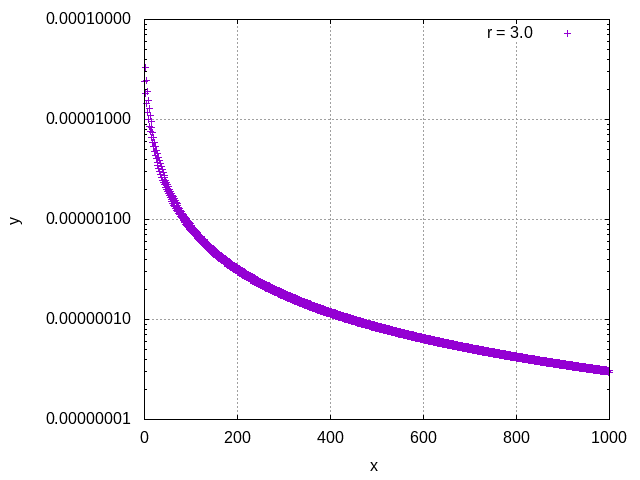
\includegraphics[width=10.0cm]{Chaosr=3_0.png}
	\label{fig:chaos_3_0}
\end{figure}


Com as variáveis definidas acima foi obtido um $\lambda$ igual a: 

\begin{equation*}
	\lambda =  -6.7051005248524717 10^{-3}
\end{equation*}

\hspace{0.5cm}

\subsubsection{Para r = 3.6}

\hspace{0.5cm}




\begin{figure}[H]
	\centering
	\caption{}{}
	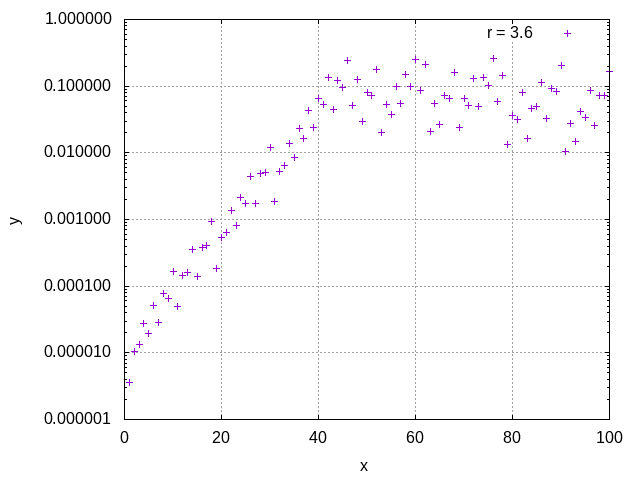
\includegraphics[width=10.0cm]{Chaosr=3_6.png}
	\label{fig:chaos_3_6}
\end{figure}

Dado que há um limite de crescimento(onde este limite é 1.0), quando a diferença se aproxima de do limite há a perda do comportamento exponencial.

\begin{equation*}
 	\lambda = 0.18498747192623105
\end{equation*}


\begin{thebibliography}{9}
\bibitem{livro}
Nicholas J Giordano - Computational Physics - Prentice Hall

\bibitem{wiki}
\url{https://en.wikipedia.org/wiki/Feigenbaum_constants} 


\end{thebibliography}
\end{document}
